\begin{center}
	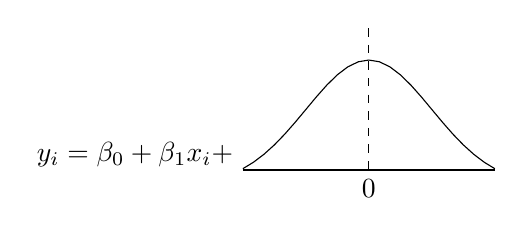
\begin{tikzpicture}[xscale = 0.8, yscale = 4]
		\coordinate (A) at (-2,0);
		\draw (A) node[left] {$y_i = \beta_0 + \beta_1 x_i + $};
		\draw [domain=-2:2] plot(\x, {exp((-(\x)^2)/2)/(sqrt(2*pi))-0.1});
		\draw [dashed] (0,0.4)--(0,-0.05);
		\draw (-2,-0.05)--(2,-0.05);
		\node (zero) at (0,-0.05)[below]{$0$};
	\end{tikzpicture}
\end{center}
